\documentclass[svgnames, 12pt]{beamer}

\usepackage[utf8]{inputenc}
\usepackage[lithuanian,english]{babel}
\usepackage[T1]{fontenc}
\usepackage{lmodern}
\usepackage{amsmath}
\usepackage{amssymb}
\usepackage{booktabs}
\usepackage{xcolor}
% \usepackage{subfig}
\usepackage{graphicx}
\usepackage{hyperref}
\usepackage{multimedia}
\usepackage{multirow}
\usepackage{tikz}
\usepackage{bm}
\usepackage{caption}
\usepackage{subcaption}
\usetikzlibrary{positioning, shapes, arrows}

% --- THEME & COLORS ---
\definecolor{mifcolor}{RGB}{0, 71, 127}
\definecolor{dimgr}{RGB}{105, 105, 105}
\definecolor{sky}{RGB}{0, 191, 255}
\setbeamercolor{alerted text}{fg=red,bg=sky}
\newcommand{\boxalert}[1]{{\usebeamercolor{alerted text}\colorbox{bg}{\alert{#1}}}}

\mode<presentation>{
  \usetheme{Madrid}
  \usecolortheme[named=mifcolor]{structure}
  \setbeamertemplate{footline}
  {%
    \leavevmode%
    \hbox{%
      \begin{beamercolorbox}[wd=.3\paperwidth,ht=2.5ex,dp=1.125ex,leftskip=.3cm
          plus1fill,rightskip=.3cm]{author in head/foot}%
        \usebeamerfont{author in head/foot}\insertshortauthor%
        \hfill
      \end{beamercolorbox}%
      \begin{beamercolorbox}[wd=.2\paperwidth,ht=2.5ex,dp=1.125ex,leftskip=.3cm,
          rightskip=.3cm plus1fil]{institute in head/foot}%
        \usebeamerfont{institute in head/foot}\insertshortinstitute%
      \end{beamercolorbox}%
      \begin{beamercolorbox}[wd=.2\paperwidth,ht=2.5ex,dp=1.125ex,leftskip=.3cm,
          rightskip=.3cm plus1fil]{date in head/foot}%
        \usebeamerfont{date in head/foot}\insertshortdate%
      \end{beamercolorbox}%
      \begin{beamercolorbox}[wd=.3\paperwidth,ht=2.5ex,dp=1.125ex,leftskip=.3cm,
          rightskip=.3cm plus1fil]{title in head/foot}%
        \usebeamerfont{title in head/foot}\insertshorttitle\hfill p.
        \insertframenumber\enspace of \inserttotalframenumber\enspace%
      \end{beamercolorbox}%
      }%
    \vskip0pt%
  }
}

\setbeamerfont{title}{size=\fontsize{17}{18}}
\title[TTS Data Strategies]{Training Data Selection Strategies for Multi-Speaker Text-to-Speech Synthesis in Lithuanian}
\subtitle{Master's Thesis Defense}
\author[A. J. Smoliakov]{Aleksandr Jan Smoliakov\inst{1}\\
  \vspace{0.4em}
  \small{Supervisor: Dr.~Gerda Ana Melnik-Leroy}\\
  \small{Scientific Advisor: Prof.~Dr.~Gražina Korvel}}
\institute[VU MIF]{\inst{1} Vilnius University, Faculty of Mathematics and Informatics}
\date{2026--01--16}

\begin{document}

\begin{frame}
  \includegraphics[scale=0.15]{MIF Garamond-logo.png}
  \hfill
  \includegraphics[scale=0.15]{Logo_spalvotas.eps}
  \titlepage%
\end{frame}

% --- PROBLEM ---
\section{Introduction}

\begin{frame}{Context \& Problem Statement}
  \begin{itemize}
    \item \textbf{Text-to-Speech (TTS)} systems (also known as speech synthesis) are widely used in virtual assistants, visual aids, and other applications.
    \item State-of-the-art \textbf{Neural TTS} typically requires 10--20 hours of
          high-quality \textit{single-speaker} data.
    \item \textbf{Low-resource languages} like Lithuanian rarely possess such datasets.
    \item \textit{Liepa-2} corpus contains 939 hours of annotated Lithuanian speech,
          but it is \textbf{fragmented} across 2,621 speakers.
    \item \textbf{Multi-speaker TTS} models can leverage such data.
    \item \textbf{Question:} What is the optimal strategy for composing multi-speaker datasets to maximize synthesis quality?
  \end{itemize}
\end{frame}

\begin{frame}{Aim \& Hypothesis}
  \begin{block}{Research Aim}
    Investigate how varying training dataset \textbf{breadth} (number of speakers) and \textbf{depth} (duration per speaker) affects the synthesis quality of multi-speaker TTS models under a constant total data budget.
  \end{block}

  \vspace{1em}
  \textbf{Hypothesis:}
  Data \textit{depth} is the critical factor. Synthesis quality will degrade as the number of speakers increases with the total training duration held constant.
\end{frame}

\begin{frame}{Research Objectives}
  \begin{enumerate}
    \item Prepare 3 subsets of \textit{Liepa-2} with varied breadth/depth but constant
          total duration.
    \item Configure and train two distinct acoustic model architectures --- one
          autoregressive (AR), one non-autoregressive (NAR).
    \item Evaluate the synthesis quality of the trained models using established
          objective evaluation metrics.
    \item Develop a subjective evaluation application and conduct listening tests to
          assess naturalness.
  \end{enumerate}
\end{frame}

% --- METHODOLOGY ---
\section{Methodology}

\begin{frame}{TTS Synthesis Pipeline}
  \begin{figure}
    \centering
    \includegraphics[width=\textwidth]{figures/tts_pipeline_mini.pdf}
  \end{figure}

  \begin{block}{TTS Synthesis Pipeline}
    A typical neural TTS pipeline. An \textbf{Acoustic model} generates Mel-spectrograms from
    input text, which are then converted to raw audio waveforms by a \textbf{Vocoder}.
  \end{block}
\end{frame}

\begin{frame}{Experimental Design: Constant ``Data Budget''}
  \begin{figure}
    \centering
    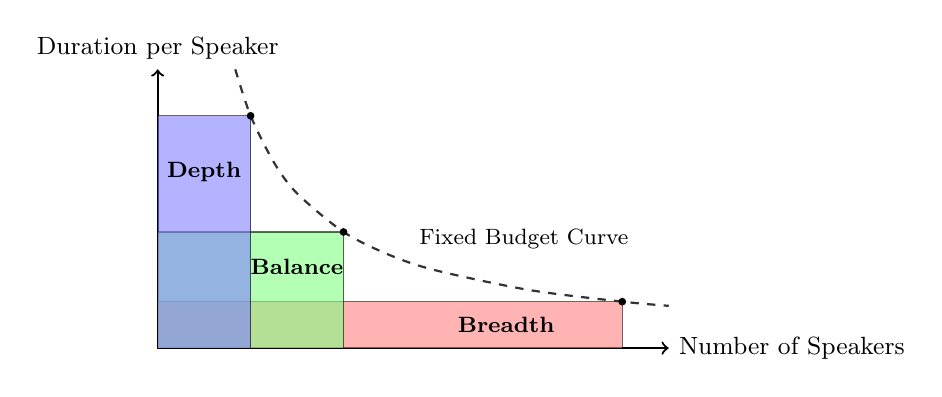
\begin{tikzpicture}[scale=0.59]
      \draw[->, thick] (0,0) -- (11,0) node[right] {\small Number of Speakers};
      \draw[->, thick] (0,0) -- (0,6) node[above] {\small Duration per Speaker};
      \draw[fill=red!50, opacity=0.6] (0,0) rectangle (10, 1);
      \node[align=center, font=\footnotesize] at (7.5, 0.5) {\textbf{Breadth}};
      \draw[fill=green!50, opacity=0.6] (0,0) rectangle (4, 2.5);
      \node[align=center, font=\footnotesize] at (3, 1.75) {\textbf{Balance}};
      \draw[fill=blue!50, opacity=0.6] (0,0) rectangle (2, 5);
      \node[align=center, font=\footnotesize] at (1, 3.8) {\textbf{Depth}};
      \draw[dashed, thick, black!80] plot [smooth] coordinates {(1.67,6) (2,5) (2.5,4) (3,3.33) (4,2.5) (5,2) (6,1.67) (8,1.25) (10,1) (11,0.91)};
      \node[above right, fill=white, inner sep=2pt, font=\footnotesize, sloped] at (5.5, 2) {Fixed Budget Curve};
      \filldraw (2,5) circle (2pt);
      \filldraw (4,2.5) circle (2pt);
      \filldraw (10,1) circle (2pt);
    \end{tikzpicture}
  \end{figure}

  Total ``data budget'' is fixed. The three strategies represent different points
  along the breadth-depth trade-off curve.
\end{frame}

\begin{frame}{Experimental Design: Constant ``Data Budget''}
  Total ``data budget'' fixed at \textbf{22.5 hours}.

  Speakers are nested (30 $\subset$ 60 $\subset$ 180) and gender-balanced to
  ensure fair comparison.

  \begin{table}[]
    \centering
    \small
    \begin{tabular}{lccc}
      \toprule
      \textbf{Strategy} & \textbf{Speakers} & \textbf{Depth/Speaker} & \textbf{Total Budget} \\
      \midrule
      \textbf{Depth}    & 30                & 45.0 min               & 22.5 h                \\
      \textbf{Balance}  & 60                & 22.5 min               & 22.5 h                \\
      \textbf{Breadth}  & 180               & 7.5 min                & 22.5 h                \\
      \bottomrule
    \end{tabular}
  \end{table}
\end{frame}

\begin{frame}{Data Preparation}
  \begin{itemize}
    \item \textbf{Source:} \textit{Liepa-2} corpus --- 939 hours of read Lithuanian speech from 2,621 speakers.
    \item \textbf{Segmentation:} Utterance-level audio segments sliced using provided timestamps.
    \item \textbf{Filtering:} Adult (18+ years) speakers only, read speech (not spontaneous).
    \item \textbf{Text:} Grapheme normalization done using rule-based preprocessing. Kirčiuoklis-based accentuation applied (where accents are unambiguous, 82\% of total words).
    \item \textbf{Audio:} Resampled to 22.05 kHz to match pre-trained vocoder.
  \end{itemize}
\end{frame}

\begin{frame}{Model Architectures}
  \begin{columns}[T]
    \begin{column}{0.5\textwidth}
      \textbf{Tacotron~2}
      \begin{itemize}
        \item Autoregressive.
        \item Seq2seq (encoder-decoder) architecture.
        \item Uses Dynamic Convolution Attention.
      \end{itemize}
    \end{column}
    \begin{column}{0.5\textwidth}
      \textbf{Glow-TTS}
      \begin{itemize}
        \item Non-autoregressive (parallel).
        \item Flow-based generative model.
        \item Uses Monotonic Alignment Search.
      \end{itemize}
    \end{column}
  \end{columns}

  \vspace{1em}
  \textbf{Speaker Embeddings:} 512-dimensional learnable embeddings, jointly trained with the acoustic models.

  \vspace{1em}
  \textbf{Vocoder:} \textit{HiFi-GAN} (pre-trained on VCTK). Frozen during training to isolate acoustic model performance.
\end{frame}

\begin{frame}{Model Training}
  \begin{itemize}
    \item \textbf{Hardware:} Personal high-performance workstation with a 48-core CPU, 256 GB of RAM, and an NVIDIA RTX 3090 GPU\@.
    \item \textbf{Hyperparameters:} Based on default configurations, with adjustments to Mel-spectrogram parameters (to match vocoder), batch size (due to hardware constraints), learning loss schedules (for a balance between convergence speed and optimal loss values), Lithuanian grapheme set, and other minor tweaks empirically found to reduce validation loss.
    \item \textbf{Training:} On each dataset, from scratch, until validation loss convergence.
          \begin{itemize}
            \item Tacotron~2 for 90k steps ($\approx 22$ hours) each.
            \item Glow-TTS for 180k steps ($\approx 25$ hours) each.
          \end{itemize}
  \end{itemize}
\end{frame}

\begin{frame}{Evaluation Setup}
  \begin{columns}[T]
    \begin{column}{0.5\textwidth}
      \textbf{Objective Metrics:}
      \begin{itemize}
        \item Mel-Cepstral Distortion (MCD): measures spectral distortion in dB.
        \item Fundamental Frequency RMSE ($F_0$ RMSE): measures pitch contour error in Hz.
      \end{itemize}
    \end{column}
    \begin{column}{0.5\textwidth}
      \textbf{Subjective Evaluation:}
      \begin{itemize}
        \item Mean Opinion Score (MOS) test
        \item 6 randomly selected speakers
        \item 60 identical test sentences for each speaker
        \item Latin Square design
      \end{itemize}
    \end{column}
  \end{columns}
\end{frame}

\begin{frame}{Evaluation Setup: Custom MOS Application}
  \begin{figure}
    \centering
    \includegraphics[width=0.65\textwidth]{figures/app_rating.png}
  \end{figure}
\end{frame}

% --- RESULTS ---
\section{Results}

\begin{frame}{Results: Alignment Convergence Examples}
  All models achieved successful \textbf{alignment convergence}.
  \vspace{0.15em}%

  \begin{figure}
    \centering

    % Tacotron 2 row
    \begin{subfigure}{0.33\textwidth}
      \centering
      \includegraphics[width=\textwidth]{figures/taco2_alignment_30spk.png}
      \caption{Tacotron~2, 30 spk}
    \end{subfigure}%
    \begin{subfigure}{0.33\textwidth}
      \centering
      \includegraphics[width=\textwidth]{figures/taco2_alignment_60spk.png}
      \caption{Tacotron~2, 60 spk}
    \end{subfigure}%
    \begin{subfigure}{0.33\textwidth}
      \centering
      \includegraphics[width=\textwidth]{figures/taco2_alignment_180spk.png}
      \caption{Tacotron~2, 180 spk}
    \end{subfigure}

    \vspace{0.15em}%

    % Glow-TTS row
    \begin{subfigure}{0.33\textwidth}
      \centering
      \includegraphics[width=\textwidth]{figures/glow_alignment_30spk.png}
      \caption{Glow-TTS, 30 spk}
    \end{subfigure}%
    \begin{subfigure}{0.33\textwidth}
      \centering
      \includegraphics[width=\textwidth]{figures/glow_alignment_60spk.png}
      \caption{Glow-TTS, 60 spk}
    \end{subfigure}%
    \begin{subfigure}{0.33\textwidth}
      \centering
      \includegraphics[width=\textwidth]{figures/glow_alignment_180spk.png}
      \caption{Glow-TTS, 180 spk}
    \end{subfigure}
  \end{figure}
\end{frame}

\begin{frame}{Results: Objective Evaluation}
  Objective metrics calculated on a 60-sentence test set (excluded from training data) by comparing synthesized audio to ground truth. Lower is better for both metrics.

  \begin{table}[]
    \centering
    \small
    \begin{tabular}{lccc}
      \toprule
      \textbf{Model}              & \textbf{Speakers} & \textbf{MCD (dB)} & \textbf{$F_0$ RMSE (Hz)} \\
      \midrule
      \multirow{3}{*}{Tacotron~2} & 30                & 9.58              & 31.28                    \\
                                  & 60                & \textbf{9.55}     & \textbf{30.49}           \\
                                  & 180               & 9.63              & 31.06                    \\
      \midrule
      \multirow{3}{*}{Glow-TTS}   & 30                & \textbf{9.90}     & 37.86                    \\
                                  & 60                & 10.00             & 36.18                    \\
                                  & 180               & 9.98              & \textbf{35.69}           \\
      \bottomrule
    \end{tabular}
  \end{table}
  \textit{Note: Minimal variation across strategies within each architecture.}
\end{frame}

\begin{frame}{Results: Subjective Naturalness (MOS)}
  Listening test with 21 native Lithuanian speakers (1,260 ratings).

  Average MOS per model architecture and data strategy shown below:

  \begin{table}[]
    \centering
    \begin{tabular}{lcc}
      \toprule
      \textbf{Strategy}                       & \textbf{Tacotron~2}                          & \textbf{Glow-TTS}        \\
      \midrule
      Depth \textit{(30 $\times$ 45.0 min)}   & 3.11 $\pm$ 0.16                              & 2.13 $\pm$ 0.12          \\
      Balance \textit{(60 $\times$ 22.5 min)} & \textbf{3.12 $\pm$ 0.17}                     & \textbf{2.18 $\pm$ 0.15} \\
      Breadth \textit{(180 $\times$ 7.5 min)} & 3.03 $\pm$ 0.18                              & 2.03 $\pm$ 0.14          \\
      \midrule
      \textbf{Ground Truth}                   & \multicolumn{2}{c}{\textbf{4.84 $\pm$ 0.06}}                            \\
      \bottomrule
    \end{tabular}
  \end{table}

  \begin{block}{Observations}
    \begin{itemize}
      \item \textbf{No significant difference} between data selection strategies within any architecture.
      \item Hypothesis: \boxalert{Rejected}.
      \item Tacotron~2 significantly outperforms Glow-TTS in naturalness.
    \end{itemize}
  \end{block}
\end{frame}

\begin{frame}{Results: Speaker-Dependent Naturalness}
  \begin{table}
    \centering
    \begin{tabular}{lcc}
      \toprule
      \textbf{Speaker ID} & \textbf{Tacotron~2 MOS} & \textbf{Glow-TTS MOS} \\
      \midrule
      AS009               & $\bm{4.17 \pm 0.20}$    & $\bm{2.61 \pm 0.23}$  \\
      IS031               & $3.26 \pm 0.20$         & $2.13 \pm 0.19$       \\
      IS038               & $3.48 \pm 0.21$         & $2.51 \pm 0.19$       \\
      MS052               & $2.26 \pm 0.17$         & $1.88 \pm 0.16$       \\
      VP131               & $2.43 \pm 0.19$         & $1.93 \pm 0.16$       \\
      VP427               & $2.92 \pm 0.22$         & $1.60 \pm 0.14$       \\
      \bottomrule
    \end{tabular}
  \end{table}

  \begin{block}{Observations}
    \textit{\href{run:Smoliakov_audio_sample_AS009.wav}{AS009}} consistently yields highest MOS scores across all models and strategies, while \textit{\href{run:Smoliakov_audio_sample_MS052.wav}{MS052}}, \textit{VP131} consistently perform poorly.

    \vspace{0.5em}
    \textbf{Qualitative analysis} revealed noticeable muffling and reverberation in \textit{MS052},
    \textit{VP131} recordings, pointing to data quality issues.
  \end{block}
\end{frame}

% --- CONCLUSIONS ---
\section{Conclusions}

\begin{frame}{Conclusions}
  \begin{enumerate}
    \item For Lithuanian multi-speaker TTS, within the tested range, the specific
          distribution of speakers does not meaningfully affect quality if the total
          budget is fixed.
    \item 7.5 minutes per speaker is sufficient for convergence of Tacotron~2 and Glow-TTS\@.
    \item Tacotron~2 outperforms Glow-TTS for naturalness in Lithuanian, likely due to
          better prosody/pitch modeling.
    \item Audio quality (reverberation, muffling) and/or speaker characteristics have a
          strong impact on synthesis naturalness.
  \end{enumerate}
\end{frame}

\begin{frame}{Recommendations \& Future Work}
  \textbf{Recommendations:}
  \begin{itemize}
    \item Prioritize maximizing \textbf{total data volume} and ensuring high per-speaker
          quality rather than optimizing the breadth-depth balance.
    \item Multi-speaker TTS models can be successfully trained from scratch using sparse
          data with 7.5 min/speaker.
  \end{itemize}

  \vspace{0.8em}
  \textbf{Future Work:}
  \begin{itemize}
    \item Investigate more architectures (e.g., VITS, FastSpeech 2).
    \item Test the ``breadth versus depth'' trade-off at higher budgets (e.g., 100+
          hours).
    \item Implement automated data quality filtering to remove muffled/reverberant
          speakers.
  \end{itemize}
\end{frame}

\begin{frame}{Thank You!}
  \begin{center}
    \vspace{2em}

    \Large Thank you for your attention!
  \end{center}
\end{frame}

\begin{frame}{Appendix 1: Reviewer's Questions}
  \begin{itemize}
    \item \textbf{Q1:} What is the purpose of a pre-processing step audio resampling process?
          \newline
    \item \textbf{Q2:} Where were the model parameters obtained or how were they selected? Were they optimal, suboptimal, or random?
          \newline
    \item \textbf{Q3:} Why the explored models (Tacotron~2 and Glow-TTS) were based on different loss function? Are these models (with different loss functions) comparable?
  \end{itemize}
\end{frame}

\begin{frame}{Appendix 2: Loss Functions}
  \textbf{Tacotron 2 optimizes Multi-component Regression Loss:}
  \begin{equation}
    \mathcal{L}_{T2} = \mathcal{L}_{Dec(L2+SSIM)} +\mathcal{L}_{Post(L2+SSIM)} + \lambda_{attn}\mathcal{L}_{Guided} + \lambda_{stop}\mathcal{L}_{Stop}
  \end{equation}

  \vspace{1em}
  \textbf{Glow-TTS optimizes Negative Log-Likelihood:}
  \begin{equation}
    \mathcal{L}_{Glow} = - \sum_{j=1}^{T_{mel}} \left[ \log \mathcal{N}(z_j; \mu, \sigma) + \log \left| \det \frac{\partial z_j}{\partial x_j} \right| \right]
  \end{equation}
\end{frame}

\begin{frame}{Appendix 3: Latin Square Design Example}
  \begin{figure}
    \centering
    \includegraphics[width=0.9\textwidth]{figures/latin_square_design.pdf}
  \end{figure}
\end{frame}

\end{document}
